%%%%%%%%%%%%%%%%%%%%%%%%%%%%%%%%%%%%%%%%%
% Important note:
% Chapter heading images should have a 2:1 width:height ratio,
% e.g. 920px width and 460px height.
%
%%%%%%%%%%%%%%%%%%%%%%%%%%%%%%%%%%%%%%%%%


%----------------------------------------------------------------------------------------
%	PACKAGES AND OTHER DOCUMENT CONFIGURATIONS
%----------------------------------------------------------------------------------------

\documentclass[openany,11pt,fleqn]{book} % Default font size and left-justified equations

\usepackage[top=3cm,bottom=3cm,left=3.2cm,right=3.2cm,headsep=10pt,letterpaper]{geometry} % Page margins

\usepackage{xcolor} % Required for specifying colors by name
\definecolor{ocre}{RGB}{52,177,201} % Define the orange color used for highlighting throughout the book

% Font Settings
\usepackage{avant} % Use the Avantgarde font for headings
%\usepackage{times} % Use the Times font for headings
\usepackage{mathptmx} % Use the Adobe Times Roman as the default text font together with math symbols from the Sym­bol, Chancery and Com­puter Modern fonts
\usepackage{microtype} % Slightly tweak font spacing for aesthetics
\usepackage[utf8]{inputenc} % Required for including letters with accents
\usepackage[T1]{fontenc} % Use 8-bit encoding that has 256 glyphs
\usepackage{amsthm}

\usepackage{circuitikz}

\usepackage{mathtools}

\usepackage{minted}

\usepackage{tikz}
\usepackage{pgfplots}
\usepgfplotslibrary{fillbetween}
\usepackage{multirow}
\usepackage{array}
\usetikzlibrary{arrows.meta, positioning, calc, trees, shapes, decorations, matrix, fit}

% Bibliography
\usepackage[style=alphabetic,sorting=nyt,sortcites=true,autopunct=true,babel=hyphen,hyperref=true,abbreviate=false,backref=true,backend=biber]{biblatex}
\addbibresource{bibliography.bib} % BibTeX bibliography file
\defbibheading{bibempty}{}
\usepackage{float}


%----------------------------------------------------------------------------------------
%	VARIOUS REQUIRED PACKAGES
%----------------------------------------------------------------------------------------

\usepackage{titlesec} % Allows customization of titles

\usepackage{graphicx} % Required for including pictures
\graphicspath{{Pictures/}} % Specifies the directory where pictures are stored
% \graphicspath{{Plots/}}
\usepackage{lipsum} % Inserts dummy text

\usepackage{tikz} % Required for drawing custom shapes

\usepackage[english]{babel} % English language/hyphenation

\usepackage{enumitem} % Customize lists
\setlist{nolistsep} % Reduce spacing between bullet points and numbered lists

\usepackage{booktabs} % Required for nicer horizontal rules in tables

\usepackage{eso-pic} % Required for specifying an image background in the title page

%----------------------------------------------------------------------------------------
%	MAIN TABLE OF CONTENTS
%----------------------------------------------------------------------------------------

\usepackage{titletoc} % Required for manipulating the table of contents

\contentsmargin{0cm} % Removes the default margin
% Chapter text styling
\titlecontents{chapter}[1.25cm] % Indentation
{\addvspace{15pt}\large\sffamily\bfseries} % Spacing and font options for chapters
{\color{ocre!60}\contentslabel[\thecontentslabel]{2cm}\color{ocre}} % Chapter number
{}  
{\color{ocre!60}\normalsize\sffamily\bfseries\;\titlerule*[.5pc]{.}\;\thecontentspage} % Page number
% Section text styling
\titlecontents{section}[1.25cm] % Indentation
{\addvspace{5pt}\sffamily\bfseries} % Spacing and font options for sections
{\contentslabel[\thecontentslabel]{1.25cm}} % Section number
{}
{\sffamily\hfill\color{black}\thecontentspage} % Page number
[]
% Subsection text styling
\titlecontents{subsection}[1.25cm] % Indentation
{\addvspace{1pt}\sffamily\small} % Spacing and font options for subsections
{\contentslabel[\thecontentslabel]{1.25cm}} % Subsection number
{}
{\sffamily\;\titlerule*[.5pc]{.}\;\thecontentspage} % Page number
[] 

%----------------------------------------------------------------------------------------
%	MINI TABLE OF CONTENTS IN CHAPTER HEADS
%----------------------------------------------------------------------------------------

% Section text styling
\titlecontents{lsection}[0em] % Indendating
{\footnotesize\sffamily} % Font settings
{}
{}
{}

% Subsection text styling
\titlecontents{lsubsection}[.5em] % Indentation
{\normalfont\footnotesize\sffamily} % Font settings
{}
{}
{}
 
%----------------------------------------------------------------------------------------
%	PAGE HEADERS
%----------------------------------------------------------------------------------------

\usepackage{fancyhdr} % Required for header and footer configuration

\pagestyle{fancy}
\renewcommand{\chaptermark}[1]{\markboth{\sffamily\normalsize\bfseries\chaptername\ \thechapter.\ #1}{}} % Chapter text font settings
\renewcommand{\sectionmark}[1]{\markright{\sffamily\normalsize\thesection\hspace{5pt}#1}{}} % Section text font settings
\fancyhf{} \fancyhead[LE,RO]{\sffamily\normalsize\thepage} % Font setting for the page number in the header
\fancyhead[LO]{\rightmark} % Print the nearest section name on the left side of odd pages
\fancyhead[RE]{\leftmark} % Print the current chapter name on the right side of even pages
\renewcommand{\headrulewidth}{0.5pt} % Width of the rule under the header
\addtolength{\headheight}{2.5pt} % Increase the spacing around the header slightly
\renewcommand{\footrulewidth}{0pt} % Removes the rule in the footer
\fancypagestyle{plain}{\fancyhead{}\renewcommand{\headrulewidth}{0pt}} % Style for when a plain pagestyle is specified

% Removes the header from odd empty pages at the end of chapters
\makeatletter
\renewcommand{\cleardoublepage}{
\clearpage\ifodd\c@page\else
\hbox{}
\vspace*{\fill}
\thispagestyle{empty}
\newpage
\fi}

%----------------------------------------------------------------------------------------
%	THEOREM STYLES
%----------------------------------------------------------------------------------------

\usepackage{amsmath,amsfonts,amssymb,amsthm} % For math equations, theorems, symbols, etc

\newcommand{\intoo}[2]{\mathopen{]}#1\,;#2\mathclose{[}}
\newcommand{\ud}{\mathop{\mathrm{{}d}}\mathopen{}}
\newcommand{\intff}[2]{\mathopen{[}#1\,;#2\mathclose{]}}
\newtheorem{notation}{Notation}[chapter]

%%%%%%%%%%%%%%%%%%%%%%%%%%%%%%%%%%%%%%%%%%%%%%%%%%%%%%%%%%%%%%%%%%%%%%%%%%%
%%%%%%%%%%%%%%%%%%%% dedicated to boxed/framed environements %%%%%%%%%%%%%%
%%%%%%%%%%%%%%%%%%%%%%%%%%%%%%%%%%%%%%%%%%%%%%%%%%%%%%%%%%%%%%%%%%%%%%%%%%%
\newtheoremstyle{ocrenumbox}% % Theorem style name
{0pt}% Space above
{0pt}% Space below
{\normalfont}% % Body font
{}% Indent amount
{\small\bf\sffamily\color{ocre}}% % Theorem head font
{\;}% Punctuation after theorem head
{0.25em}% Space after theorem head
{\small\sffamily\color{ocre}\thmname{#1}\nobreakspace\thmnumber{\@ifnotempty{#1}{}\@upn{#2}}% Theorem text (e.g. Theorem 2.1)
\thmnote{\nobreakspace\the\thm@notefont\sffamily\bfseries\color{black}---\nobreakspace#3.}} % Optional theorem note
\renewcommand{\qedsymbol}{$\blacksquare$}% Optional qed square

\newtheoremstyle{blacknumex}% Theorem style name
{5pt}% Space above
{5pt}% Space below
{\normalfont}% Body font
{} % Indent amount
{\small\bf\sffamily}% Theorem head font
{\;}% Punctuation after theorem head
{0.25em}% Space after theorem head
{\small\sffamily{\tiny\ensuremath{\blacksquare}}\nobreakspace\thmname{#1}\nobreakspace\thmnumber{\@ifnotempty{#1}{}\@upn{#2}}% Theorem text (e.g. Theorem 2.1)
\thmnote{\nobreakspace\the\thm@notefont\sffamily\bfseries---\nobreakspace#3.}}% Optional theorem note

\newtheoremstyle{blacknumbox} % Theorem style name
{0pt}% Space above
{0pt}% Space below
{\normalfont}% Body font
{}% Indent amount
{\small\bf\sffamily}% Theorem head font
{\;}% Punctuation after theorem head
{0.25em}% Space after theorem head
{\small\sffamily\thmname{#1}\nobreakspace\thmnumber{\@ifnotempty{#1}{}\@upn{#2}}% Theorem text (e.g. Theorem 2.1)
\thmnote{\nobreakspace\the\thm@notefont\sffamily\bfseries---\nobreakspace#3.}}% Optional theorem note

%%%%%%%%%%%%%%%%%%%%%%%%%%%%%%%%%%%%%%%%%%%%%%%%%%%%%%%%%%%%%%%%%%%%%%%%%%%
%%%%%%%%%%%%% dedicated to non-boxed/non-framed environements %%%%%%%%%%%%%
%%%%%%%%%%%%%%%%%%%%%%%%%%%%%%%%%%%%%%%%%%%%%%%%%%%%%%%%%%%%%%%%%%%%%%%%%%%
\newtheoremstyle{ocrenum}% % Theorem style name
{5pt}% Space above
{5pt}% Space below
{\normalfont}% % Body font
{}% Indent amount
{\small\bf\sffamily\color{ocre}}% % Theorem head font
{\;}% Punctuation after theorem head
{0.25em}% Space after theorem head
{\small\sffamily\color{ocre}\thmname{#1}\nobreakspace\thmnumber{\@ifnotempty{#1}{}\@upn{#2}}% Theorem text (e.g. Theorem 2.1)
\thmnote{\nobreakspace\the\thm@notefont\sffamily\bfseries\color{black}---\nobreakspace#3.}} % Optional theorem note
\renewcommand{\qedsymbol}{$\blacksquare$}% Optional qed square
\makeatother

% Defines the theorem text style for each type of theorem to one of the three styles above
\newcounter{dummy} 
\numberwithin{dummy}{section}
\theoremstyle{ocrenumbox}


\newtheorem{theoremeT}[dummy]{Theorem}
\newtheorem{lemma}[dummy]{Lemma}
\newtheorem{observation}[dummy]{Observation}
\newtheorem{proposition}[dummy]{Proposition}
% \newtheorem{definition}[dummy]{Definition}
\newtheorem{claim}[dummy]{Claim}
\newtheorem{fact}[dummy]{Fact}
\newtheorem{assumption}[dummy]{Assumption}

\newtheorem{problem}{Problem}[chapter]
% \newtheorem{exercise}{Exercise}[chapter]
\theoremstyle{blacknumex}
\newtheorem{exampleT}{Example}[chapter]
\theoremstyle{blacknumbox}
\newtheorem{vocabulary}{Vocabulary}[chapter]
\newtheorem{definitionT}{Definition}[section]
\newtheorem{corollaryT}[dummy]{Corollary}
\theoremstyle{ocrenum}



%----------------------------------------------------------------------------------------
%	DEFINITION OF COLORED BOXES
%----------------------------------------------------------------------------------------

\RequirePackage[framemethod=default]{mdframed} % Required for creating the theorem, definition, exercise and corollary boxes

% Theorem box
\newmdenv[skipabove=7pt,
skipbelow=7pt,
backgroundcolor=black!5,
linecolor=ocre,
innerleftmargin=5pt,
innerrightmargin=5pt,
innertopmargin=5pt,
leftmargin=0cm,
rightmargin=0cm,
innerbottommargin=5pt]{tBox}

% Exercise box	  
\newmdenv[skipabove=7pt,
skipbelow=7pt,
rightline=false,
leftline=true,
topline=false,
bottomline=false,
backgroundcolor=ocre!10,
linecolor=ocre,
innerleftmargin=5pt,
innerrightmargin=5pt,
innertopmargin=5pt,
innerbottommargin=5pt,
leftmargin=0cm,
rightmargin=0cm,
linewidth=4pt]{eBox}	

% Definition box
\newmdenv[skipabove=7pt,
skipbelow=7pt,
rightline=false,
leftline=true,
topline=false,
bottomline=false,
linecolor=ocre,
innerleftmargin=5pt,
innerrightmargin=5pt,
innertopmargin=0pt,
leftmargin=0cm,
rightmargin=0cm,
linewidth=4pt,
innerbottommargin=0pt]{dBox}	

% Corollary box
\newmdenv[skipabove=7pt,
skipbelow=7pt,
rightline=false,
leftline=true,
topline=false,
bottomline=false,
linecolor=gray,
backgroundcolor=black!5,
innerleftmargin=5pt,
innerrightmargin=5pt,
innertopmargin=5pt,
leftmargin=0cm,
rightmargin=0cm,
linewidth=4pt,
innerbottommargin=5pt]{cBox}

% Creates an environment for each type of theorem and assigns it a theorem text style from the "Theorem Styles" section above and a colored box from above
\newenvironment{theorem}{\begin{tBox}\begin{theoremeT}}{\end{theoremeT}\end{tBox}}
\newenvironment{exercise}{\begin{eBox}\begin{exerciseT}}{\hfill{\color{ocre}\tiny\ensuremath{\blacksquare}}\end{exerciseT}\end{eBox}}				  
\newenvironment{definition}{\begin{dBox}\begin{definitionT}}{\end{definitionT}\end{dBox}}	
\newenvironment{example}{\begin{exampleT}}{\hfill{\tiny\ensuremath{\blacksquare}}\end{exampleT}}		
\newenvironment{corollary}{\begin{cBox}\begin{corollaryT}}{\end{corollaryT}\end{cBox}}	

%----------------------------------------------------------------------------------------
%	REMARK ENVIRONMENT
%----------------------------------------------------------------------------------------

\newenvironment{remark}{\par\vspace{10pt}\small % Vertical white space above the remark and smaller font size
\begin{list}{}{
\leftmargin=35pt % Indentation on the left
\rightmargin=25pt}\item\ignorespaces % Indentation on the right
\makebox[-2.5pt]{\begin{tikzpicture}[overlay]
\node[draw=ocre!60,line width=1pt,circle,fill=ocre!25,font=\sffamily\bfseries,inner sep=2pt,outer sep=0pt] at (-15pt,0pt){\textcolor{ocre}{R}};\end{tikzpicture}} % Orange R in a circle
\advance\baselineskip -1pt}{\end{list}\vskip5pt} % Tighter line spacing and white space after remark

%----------------------------------------------------------------------------------------
%	SECTION NUMBERING IN THE MARGIN
%----------------------------------------------------------------------------------------

\makeatletter
\renewcommand{\@seccntformat}[1]{\llap{\textcolor{ocre}{\csname the#1\endcsname}\hspace{1em}}}                    
\renewcommand{\section}{\@startsection{section}{1}{\z@}
{-4ex \@plus -1ex \@minus -.4ex}
{1ex \@plus.2ex }
{\normalfont\large\sffamily\bfseries}}
\renewcommand{\subsection}{\@startsection {subsection}{2}{\z@}
{-3ex \@plus -0.1ex \@minus -.4ex}
{0.5ex \@plus.2ex }
{\normalfont\sffamily\bfseries}}
\renewcommand{\subsubsection}{\@startsection {subsubsection}{3}{\z@}
{-2ex \@plus -0.1ex \@minus -.2ex}
{.2ex \@plus.2ex }
{\normalfont\small\sffamily\bfseries}}                        
\renewcommand\paragraph{\@startsection{paragraph}{4}{\z@}
{-2ex \@plus-.2ex \@minus .2ex}
{.1ex}
{\normalfont\small\sffamily\bfseries}}

%----------------------------------------------------------------------------------------
%	HYPERLINKS IN THE DOCUMENTS
%----------------------------------------------------------------------------------------

% For an unclear reason, the package should be loaded now and not later
\usepackage{hyperref}
\hypersetup{hidelinks,backref=true,pagebackref=true,hyperindex=true,colorlinks=false,breaklinks=true,urlcolor= ocre,bookmarks=true,bookmarksopen=false,pdftitle={Title},pdfauthor={Author}}

%----------------------------------------------------------------------------------------
%	CHAPTER HEADINGS
%----------------------------------------------------------------------------------------

% The set-up below should be (sadly) manually adapted to the overall margin page septup controlled by the geometry package loaded in the main.tex document. It is possible to implement below the dimensions used in the goemetry package (top,bottom,left,right)... TO BE DONE

\newcommand{\thechapterimage}{}
\newcommand{\chapterimage}[1]{\renewcommand{\thechapterimage}{#1}}

% Numbered chapters with mini tableofcontents
\def\thechapter{\arabic{chapter}}
\def\@makechapterhead#1{
\thispagestyle{empty}
{\centering \normalfont\sffamily
\ifnum \c@secnumdepth >\m@ne
\if@mainmatter
\startcontents
\begin{tikzpicture}[remember picture,overlay]
\node at (current page.north west)
{\begin{tikzpicture}[remember picture,overlay]
\node[anchor=north west,inner sep=0pt] at (0,0) {\includegraphics[width=\paperwidth]{\thechapterimage}};
%%%%%%%%%%%%%%%%%%%%%%%%%%%%%%%%%%%%%%%%%%%%%%%%%%%%%%%%%%%%%%%%%%%%%%%%%%%%%%%%%%%%%
% Commenting the 3 lines below removes the small contents box in the chapter heading
%\fill[color=ocre!10!white,opacity=.6] (1cm,0) rectangle (8cm,-7cm);
%\node[anchor=north west] at (1.1cm,.35cm) {\parbox[t][8cm][t]{6.5cm}{\huge\bfseries\flushleft \printcontents{l}{1}{\setcounter{tocdepth}{2}}}};
\draw[anchor=west] (5cm,-9cm) node [rounded corners=20pt,fill=ocre!10!white,text opacity=1,draw=ocre,draw opacity=1,line width=1.5pt,fill opacity=.6,inner sep=12pt]{\Large\sffamily\bfseries\textcolor{black}{\thechapter. #1\strut\makebox[22cm]{}}};
%%%%%%%%%%%%%%%%%%%%%%%%%%%%%%%%%%%%%%%%%%%%%%%%%%%%%%%%%%%%%%%%%%%%%%%%%%%%%%%%%%%%%
\end{tikzpicture}};
\end{tikzpicture}}
\vskip 223pt % Changed to \vskip from \par\vspace*{} bc it was skipping pages for me
\fi
\fi}

% Unnumbered chapters without mini tableofcontents (could be added though) 
\def\@makeschapterhead#1{
\thispagestyle{empty}
{\centering \normalfont\sffamily
\ifnum \c@secnumdepth >\m@ne
\if@mainmatter
\begin{tikzpicture}[remember picture,overlay]
\node at (current page.north west)
{\begin{tikzpicture}[remember picture,overlay]
\node[anchor=north west,inner sep=0pt] at (0,0) {\includegraphics[width=\paperwidth]{\thechapterimage}};
\draw[anchor=west] (5cm,-9cm) node [rounded corners=20pt,fill=ocre!10!white,fill opacity=.6,inner sep=12pt,text opacity=1,draw=ocre,draw opacity=1,line width=1.5pt]{\huge\sffamily\bfseries\textcolor{black}{#1\strut\makebox[22cm]{}}};
\end{tikzpicture}};
\end{tikzpicture}}
\vskip 223pt % Changed to \vskip from \par\vspace*{} bc it was skipping pages for me
\fi
\fi
}
\makeatother % Insert the commands.tex file which contains the majority of the structure behind the template

%----------------------------------------------------------------------------------------
%	Definitions of new commands
%----------------------------------------------------------------------------------------

\newcounter{ttl@toc@default} % Add counter definition

\newcommand{\cvx}{convex}
\thinmuskip=6mu
\medmuskip=8mu plus 4mu minus 6mu
\thickmuskip=10mu plus 10mu
\setlength{\parindent}{0pt} % Remove paragraph indentation
\setlength{\parskip}{0pt} % Remove paragraph skip
\allowdisplaybreaks

\includeonly{
    % LECTURE_1/lecture_1.tex,
    % LECTURE_2/lecture_2.tex,
    % LECTURE_3/lecture_3.tex,
    LECTURE_4/lecture_4.tex,
    % LECTURE_5/lecture_5.tex,
    % LECTURE_6/lecture_6.tex
}

\begin{document}

\renewcommand{\thedummy}{\Roman{chapter}.\Roman{section}.\Roman{dummy}}
\renewcommand{\thedefinitionT}{\Roman{chapter}.\Roman{section}.\Roman{definitionT}}
\renewcommand{\theexampleT}{\Roman{chapter}.\Roman{exampleT}}
\renewcommand{\thechapter}{Lecture \Roman{chapter}} % Chapter numbering in Roman numerals
\renewcommand{\thesection}{\Roman{chapter}.\Roman{section}} % Section numbering in Roman numerals
\renewcommand{\thesubsection}{\Roman{chapter}.\Roman{section}.\Roman{subsection}} % Subsection numbering in Roman numerals
\renewcommand{\thetable}{\Roman{chapter}.\Roman{table}}
\renewcommand{\theequation}{\Roman{chapter}.\Roman{equation}}
\renewcommand{\theproblem}{\Roman{problem}}


%----------------------------------------------------------------------------------------
%	TITLE PAGE
%----------------------------------------------------------------------------------------

\begingroup
\thispagestyle{empty}
\AddToShipoutPicture*{\put(0,0){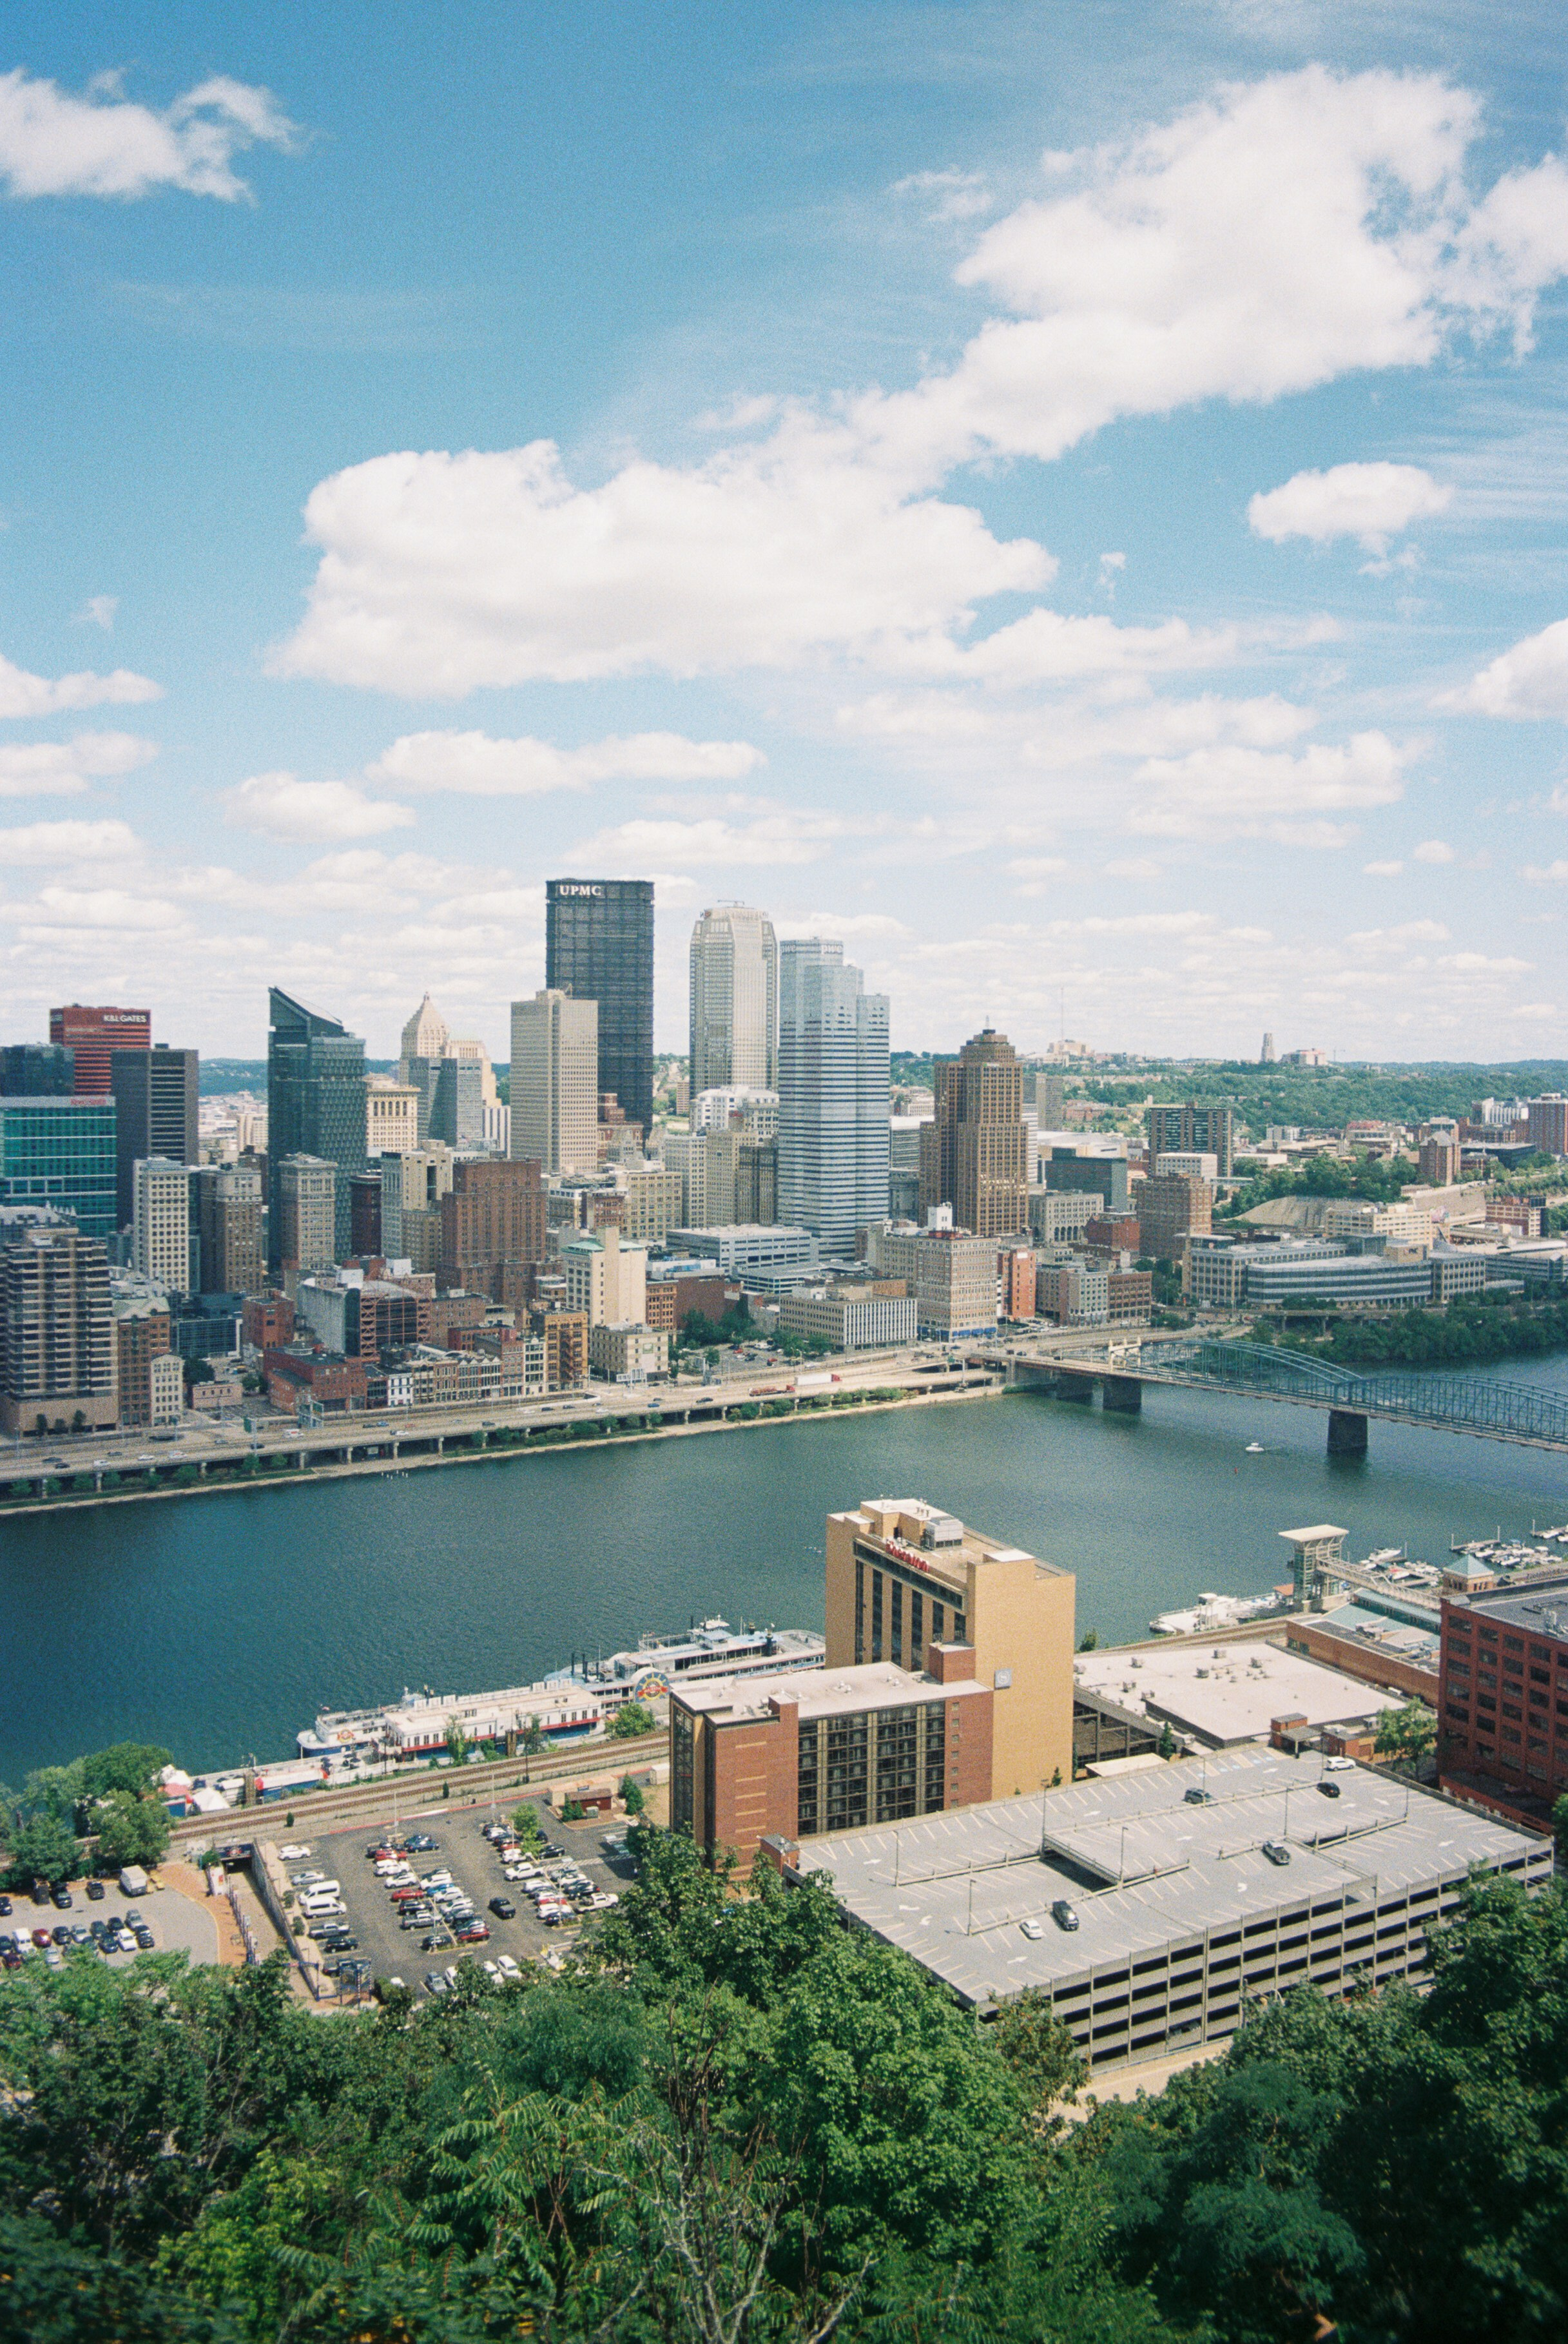
\includegraphics[scale=0.385]{./Images/banner.jpg}}} % Image background
\centering
\vspace*{5cm}
\par\normalfont\fontsize{35}{35}\sffamily\selectfont
\textbf{ECE349H1 Fall 2024}\\
{\LARGE Introduction to Energy Systems}\par % Book title
\vspace*{1cm}
{\Huge Nasrudeen Oladimeji}\par % Author name
\endgroup

%----------------------------------------------------------------------------------------
%	COPYRIGHT PAGE
%----------------------------------------------------------------------------------------

\newpage
~\vfill
\thispagestyle{empty}

%\noindent Copyright \copyright\ 2014 Andrea Hidalgo\\ % Copyright notice

\noindent\textsc{University of Toronto}\\

\noindent \textsc{github.com/Nasr-905}\\ % URL

\noindent Professor: \\ % License information

\noindent \textit{First release, September 2024} % Printing/edition date

%----------------------------------------------------------------------------------------
%	TABLE OF CONTENTS
%----------------------------------------------------------------------------------------

\chapterimage{./Images/head1.jpg} % Table of contents heading image

\pagestyle{empty} % No headers

\tableofcontents % Print the table of contents itself

%\cleardoublepage % Forces the first chapter to start on an odd page so it's on the right

\pagestyle{fancy} % Print headers again

% theorem
% problem
% example
% vocabulary
% definition
% corollary
% remark
% proof
% lemma
% observation
% proposition
% claim
% fact
% assumption


% \chapterimage{./Images/head2.jpg} % Chapter heading image
\chapter{The Introduction}


% \chapterimage{./Images/head2.jpg} % Chapter heading image
\chapter{AC Steady State Analysis (Thomas + Rosa 669-689)}


\begin{vocabulary}
    [Phasor]
    Phasors solve \textit{linear} circuits with sinusoidal sources. We can use phasors to solve circuits with \textit{time-varying} sources, but we need to convert the time-varying sources to phasors first.
\end{vocabulary}
\begin{remark}
    Linear Differential Equation have solutions with two parts:
    \begin{itemize}
        \item Homogenous solution: Response to initial conditions
        \item Particular solution: Response to forcing function
    \end{itemize}
    Since they're linear, we can add the two solutions together using \textbf{superposition} to get the total solution.
\end{remark}

\begin{corollary}
    [Stable Systems]
    For stable systems (e.g. passive) circuits:
    \[
        \text{Homogenous solution} \to 0 \text{ as } t \to \infty
    \]
\end{corollary}

\begin{remark}
    Phasor analysis is the fastest way to get a \textit{particular solution} for a circuit with sinusoidal sources.
\end{remark}

\begin{example}
    [INSERT IMAGE FROM PHONE]
    Find $i(t)$ after transient decay.\\
    \begin{align}
        Ri & + L\frac{di}{dt}= V \cos(\omega t \phi)                           \\
           & Vcos(\omega t \phi) = Re{\{Ve^{j(\omega t + \phi)} = \tilde{V}\}} \\
    \end{align}
    Find $\tilde{I}$ from:
    \[
        R \tilde{I} + L\frac{d\tilde{I}}{dt} = \tilde{V}
    \]
    Then take real part of $\tilde{I}$ to get $i(t)$.\\
    \textbf{General for of solution:}
    \[
        \tilde{I} = \textbf{I}e^{j\omega t} \quad \text{where } \textbf{I} \text{ is a complex number without time dependence (doesn't contain)} e^{j\omega t}
    \]
    Substitute into the differential equation:
    \[
        R\textbf{I}e^{j\omega t} + Lj\omega \textbf{I}e^{j\omega t} = Ve^{j\omega t + \phi}
    \]
    Find $\textbf{I}$ by cancelling $e^{j\omega t}$ terms:
    \[
        R \textbf{I} + j\omega L \textbf{I}= Ve^{j\phi} = \textbf{V} \quad \text{Voltage phasor}
    \]
    \begin{align}
        \textbf{I} & = \frac{\textbf{V}}{R + j\omega L}                                                                            \\
        \textbf{I} & = \frac{V}{\sqrt{R^2 + (\omega L)^2}}\angle{\phi - \tan^{-1} \frac{\omega L}{R}} \quad  \text{Current phasor} \\
        \tilde{I}  & = \textbf{I}e^{j\omega t}                                                                                     \\
        \tilde{I}  & = \frac{|V|}{\sqrt{R^2 + (\omega L)^2}}e^{j\omega t + \phi - \tan^{-1} \frac{\omega L}{R}}
    \end{align}
    Now we can reconstruct $i(t)$:
    \begin{align}
        i(t) & = \Re\{\tilde{I}\} = \Re\left\{\frac{|V|}{\sqrt{R^2 + (\omega L)^2}}e^{j\omega t + \phi - \tan^{-1} \frac{\omega L}{R}}\right\} \\
             & = \frac{|V|}{\sqrt{R^2 + (\omega L)^2}}\cos(\omega t + \phi - \tan^{-1} \frac{\omega L}{R})
    \end{align}
\end{example}

\begin{remark}
    In practice, skip \textit{intermediate} variables $\tilde{i}$ and $\tilde{V}$
\end{remark}

\subsection*{Steps for Phasor Analysis}
\begin{enumerate}
    \item Defiune phasors $V\cos(\omega t + \phi) \iff V\angle{\phi}$
    \item Map L's and C's to impedances \begin{align}
              v  = L\frac{di}{dt}   & \iff \textbf{V} = j\omega L \textbf{I}      \\
              i = C\frac{dv}{dt}    & \iff \textbf{I} = j\omega C \textbf{V}      \\
              \text{or equivalent } & \textbf{V} = \frac{1}{j\omega C} \textbf{I}
          \end{align}
    \item Mesh (or Nodal) analysis for phasor solution
    \item Recreate time-domain solution from phasor solution (e.g. get $i(t)$ from $\textbf{{I}}$)
\end{enumerate}

\begin{observation}
    [Converting from Time to Phasor Domain]
    \begin{align}
        V\cos(\omega t + \phi) & \iff \textbf{V} = V\angle{\phi} \\
        I\cos(\omega t + \phi) & \iff \textbf{I} = I\angle{\phi}
    \end{align}
\end{observation}

\begin{example}
    [Example 2]
    Find the steady state solution for $i(t)$ in the circuit below:

    \begin{enumerate}
        \item Step 1: Define phasors
              \[                  v(t) = 1\cos(10 t) \iff \textbf{V} = 1\angle{0}
              \]
        \item Step 2: Map L's and C's to impedances \begin{align}
                  R = 1 \quad L = j\omega 1 \quad C = \frac{1}{j\omega 0.1} \\
              \end{align}
        \item Step 3: Mesh analysis for phasor solution
              \begin{align}
                  \textbf{I} & = \frac{1\angle{0}}{1 + j(10)(1) + \frac{1}{j(10)(0.1)}} \\
                             & = 0.11 \angle{-83^\circ}
              \end{align}
        \item Step 4: Recreate time-domain solution from phasor solution \[i(t) = 0.11\cos(10t - 83^\circ)\]
    \end{enumerate}
\end{example}

\section{Frequency Response}
\begin{example}
    THIRD IMAGE

    Find $\textbf{V_0}$ as a function of $\textbf{V_i}$ and $w$
    \begin{align}
        \textbf{V_0}                           & = \frac{1/j\omega C}{R + 1/....}\textbf{V_i} \\
        \textbf{\textnormal{\frac{V_0}{V_i} }} & = \frac{1}{1 + j\omega RC}
    \end{align}
    Now we can plot the magnitude and phase of $\textbf{V_0}/\textbf{V_i}$ as a function of $\omega$ on a log-log plot.
    FOURTH IMAGE
    Essentially we made a low-pass filter, and characterized it's frequency response.
\end{example}




% \chapter{Superposition and Power}
\section{Superposition}
\begin{theorem}
    [Superposition]
    The response of a linear circuit to a sum of sources is the sum of the responses to each source acting alone, \textit{even if the sources have different frequencies}.
\end{theorem}

\begin{example}
    INSERT IMAGE FROM PHONE\\
    Solve at $100 rad/s$
    \begin{align}
        \underline{I_1} = \frac{100 \angle{0}}{100 + j100} = 0.707 \angle{-45^\circ} \\
        i_1(t) = 0.707\cos(100t - 45^\circ)
    \end{align}
    INSERT IMAGE FROM PHONE\\
    Solve at $200 rad/s$
    \begin{align}
        \underline{I_2} = \frac{100 \angle{0}}{100 + j200}\times 2\angle{0} = 0.894\angle{-63^\circ} \\
        i_2(t) = 0.894\cos(200t - 63^\circ)
    \end{align}
    INSERT IMAGE FROM PHONE\\
    Super impose in the time-domain. \\
    \begin{align}
        i(t) & = i_1(t) + i_2(t)                                         \\
             & = 0.707\cos(100t - 45^\circ) + 0.894\cos(200t - 63^\circ)
    \end{align}
\end{example}

\section{Periodic Non-Sinusoidal Systems}
\begin{remark}
    Periodic stimuli can be converted into sinusoidal stimuli using \textbf{Fourier analysis.}
\end{remark}
\begin{example}
    [Square Wave]
    \begin{align}
        v_s(t) & = a_0 \sum a_k \cos(k\omega t) + \sum b_k \sin(k\omega t) \\
        a_0    & = \frac{1}{T}\int_{0}^{T}v_s(t)dt                         \\
        a_k    & = \frac{2}{T}\int_{0}^{T}v_s(t)\cos(k\omega t)dt          \\
        b_k    & = \frac{2}{T}\int_{0}^{T}v_s(t)\sin(k\omega t)dt
    \end{align}
\end{example}
\begin{figure}[h]
    \centering
    \begin{tikzpicture}
        \draw[->] (0,0) -- (5,0) node[right] {$t$};
        \draw[->] (0,0) -- (0,2) node[above] {$V$};
        \draw[thick] (0,1) -- (1,1) -- (1,-1) -- (2,-1) -- (2,1) -- (3,1) -- (3,-1) -- (4,-1) -- (4,1) -- (5,1);
    \end{tikzpicture}
    \caption{Square wave}
\end{figure}

\begin{example}
    [Square Wave 2]
    Say we wanted to solve \ref{fig:Square wave circuit} with a square wave source. We can use superposition of an infinite number of sinusoidal sources to solve this circuit.
\end{example}
% tikz circuit with square source, resistor and inductor
\begin{figure}[h]
    \centering
    \begin{circuitikz}
        \draw (0,0) to[sV, l=$Square wave$] (0,2) to[R, l=$R$] (2,2) to[L, l=$L$] (2,0) -- (0,0);
    \end{circuitikz}
    \caption{Square wave circuit}
\end{figure}

\section{Power}
\begin{definition}
    [Instantaneous Power]
    The instantaneous power is the product of the instantaneous voltage and current.
    \[
        p(t) = v(t)i(t)
    \]
    AC source on resistor
\end{definition}
\begin{example}
    [Power in resistor]
    \begin{align}
        v(t) & = V\cos(\omega t)                                                   \\
        i(t) & = I\cos(\omega t)                                                   \\
        p(t) & = V\cos(\omega t)I\cos(\omega t) = \frac{VI}{2}(1 +\cos(2\omega t))
    \end{align}
\end{example}
\begin{figure}[h]
    \centering
    \begin{circuitikz}
        \draw (0,0) to[sV, l=$\hat{V}\cos{\omega t}$] (0,2) to[R, l=$R$] (2,2) to[short, l=$\hat{I}\cos{\omega t}$] (2,0) -- (0,0);
    \end{circuitikz}
    \caption{Power in resistor}
\end{figure}

\begin{definition}
    [Average Power]
    The average power is the time average of the instantaneous power.
    \[
        P = \frac{1}{T}\int_{0}^{T}p(t)dt
    \]
\end{definition}
% Tikz graph showing sinuoidal source and average power
\begin{definition}
    [Rective Power]
    The reactive power is the imaginary part of the complex power.
\end{definition}

\begin{remark}
    $\hat{I}, \hat{V}$ are phasors. The peak values of the sinusoidal source.
\end{remark}

let $\phi = \angle{V} - \angle{I}$

\begin{example}
    [Reactive Power]
    \begin{align}
        p(t) & = \hat{V}\cos(\omega t)\hat{I}\cos(\omega t - \phi)                                                             \\
             & = \frac{\hat{V}\hat{I}}{2}(\cos(\phi) + \cos(2\omega t + \phi))                                                 \\
             & = \frac{\hat{V}\hat{I}}{2}\cos(\phi(1 + \cos(2\omega t)) - \frac{\hat{V}\hat{I}}{2}\sin(\phi)(\sin(2\omega t))) \\
    \end{align}
    We get less real power if $\hat{V}$ and $\hat{I}$ are out of phase.
\end{example}

\chapter{Power}

\section{Average Power}

\begin{definition}
    [Average Power]
    The average power is the time average of the instantaneous power.
    \begin{align}
        p(t) & = v(t)i(t)                                                                                                                     \\
        P    & = \frac{1}{T}\int_{0}^{T}p(t)dt                                                                                                \\
        P    & = \frac{1}{T}\int_{0}^{T}\frac{\hat{V}\hat{I}}{2}(\cos(1 + 2\omega t)) + \frac{\hat{V}\hat{I}}{2}\sin(\phi)(\sin(2\omega t))dt \\ \text{Just use this } P & = \frac{\hat{V}\hat{I}}{2}\cos(\phi)
    \end{align}
    The first term is the real power and the second term is the reactive power (in/out of storage element).
\end{definition}

\begin{definition}
    [Reactive Power]
    Measure of energy going in/out of storage element. Essentially, the imaginary part of the complex power.
    \begin{align}
        Q \triangleq \frac{\hat{V}\hat{I}}{2}\sin(\phi)
    \end{align}
\end{definition}

\section{Displacement Factor}
\begin{definition}
    [Displacement Factor]
    The displacement factor is the cosine of the phase difference between the voltage and current. Essentially a measure of the angle between the voltage and current.
    \begin{align}
        \text{DF} \triangleq \cos(\phi)
    \end{align}
    \textit{$DF = 1$ means the voltage and current are in phase and you get the most real power.}
\end{definition}

\begin{remark}
    As a power company, you want to have a high displacement factor to reduce the amount of reactive power you have to supply. Increasing the amperage, you would need thicker wires and more expensive equipment, so you want to maximize $W/A$.
\end{remark}

\begin{example}
    [Displacement Factor]
    \begin{align}
        \text{DF} & = 0.866 \implies \phi = \pm 30^{\circ} \\
    \end{align}
\end{example}
\begin{vocabulary}
    [Lagging/Leading Power Factor]
    \begin{align}
        \text{Lagging} & : \phi > 0 \hat{I} \quad \text{lags}\quad  \hat{V}          \\
        \text{Leading} & : \phi < 0 \hat{I} \quad \text{leads}\quad  \hat{V}         \\
        \text{Unity}   & : \phi = 0 \hat{I} \quad \text{in phase with}\quad  \hat{V}
    \end{align}
\end{vocabulary}

% tikz graph polar plot of power factor
\begin{figure}
    \centering
    \begin{tikzpicture}
        % polar plot of voltage and current
        \draw[->] (0,0) -- (0,3) node[anchor=south] {$\hat{V}$};
        \draw[->] (0,0) -- (3,0) node[anchor=west] {$\hat{I}$};
        \draw[->] (0,0) -- (2.6,2.6) node[anchor=south west] {$\hat{S}$};
        \draw[->] (0,0) -- (2.6,0) node[anchor=north] {$\hat{P}$};
        \draw[->] (0,0) -- (0,2.6) node[anchor=east] {$\hat{Q}$};
    \end{tikzpicture}
\end{figure}

\section{P \& Q from Phasors}

\begin{definition}
    [Complex Power]
    \begin{align}
        P & = \frac{\hat{V}\hat{I}}{2}\cos(\phi_{V} - \phi_{I})           \\
          & = \frac{1}{2}\hat{V}\hat{I}\Re{e^{j\phi_{V}}e^{-j\phi_{I}}}   \\
          & = \frac{1}{2}\Re{[\hat{V}e^{j\phi_{V}}\hat{I}e^{-j\phi_{I}}]} \\
          & = \frac{1}{2}\Re[{\hat{V}\cdot \hat{I}^{*}}]                  \\
    \end{align}

    \begin{align}
        Q & = \frac{\hat{V}\hat{I}}{2}\sin(\phi_{V} - \phi_{I})           \\
          & = \frac{1}{2}\hat{V}\hat{I}\Im{e^{j\phi_{V}}e^{-j\phi_{I}}}   \\
          & = \frac{1}{2}\Im{[\hat{V}e^{j\phi_{V}}\hat{I}e^{-j\phi_{I}}]} \\
          & = \frac{1}{2}\Im[{\hat{V}\cdot \hat{I}^{*}}]                  \\
    \end{align}
    So we define:
    \begin{align}
        S & = \frac{1}{2}(\hat{\underline{V}}\cdot \hat{\underline{I}}^{*}) \qquad \frac{1}{2}\text{ because we use peak values} \\
          & = P + jQ                                                                                                             \\
        P & = \Re{S}                                                                                                             \\
        Q & = \Im{S}
    \end{align}
\end{definition}

\begin{remark}
    Review Thomas/Rose 16.1 to 16.3 for more information on complex power.
\end{remark}

\subsection{Root Mean Square (RMS) Values (Erickson E.d. 2: 16.2, E.d.3 20.2)}

\begin{theorem}
    \begin{align}
        p(t) & = v(t)i(t)                                       \\
             & = v(t) \cdot \frac{v(t)}{R}                      \\
             & = \frac{v^{2}(t)}{R}                             \\
             & = \frac{1}{R}[\frac{1}{T}\int_{0}^{T}v^{2}(t)dt] \\
    \end{align}
    We want to find a way to relate the average power to the $v^2(t)$ (or $i^2(t)$), without worrying about whether it's a sine wave, square wave, etc. Using RMS values allows us to treat all signals the same.
    \begin{align}
        V_{rms} & = \sqrt{\frac{1}{T}\int_{0}^{T}v^{2}(t)dt} \\
        I_{rms} & = \sqrt{\frac{1}{T}\int_{0}^{T}i^{2}(t)dt}
    \end{align}
\end{theorem}

\begin{definition}
    [RMS Values]
    Measure of \textit{\textbf{average power}} and \textit{\textbf{periodic signal}} of a sinusoidal signal.
    \begin{align}
        P = \frac{1}{R}v_{rms}^{2} \\
        P = \frac{1}{R}i_{rms}^{2}
    \end{align}
\end{definition}

\section{RMS of Sinusoidal Signals}

\begin{proof}
    \begin{align}
        v_{rms} & = \sqrt{\frac{1}{2\pi}\int_{0}^{2\pi}\hat{V}^{2}\sin^{2}(\omega t)dt}                \\
        v_{rms} & = \frac{1}{\sqrt{2}}\hat{V} \qquad \text{ \textbf{ONLY} for pure sinusoidal signals}
    \end{align}
\end{proof}

\begin{example}
    [RMS of Sinusoidal Superpositions]
    If
    \begin{align}
        v(t)                     & = v_0 + \hat{V_1}\cos{(\omega t + \phi_1)} + \hat{V_2}\cos{(\omega t + \phi_2)} \\
        v_{rms}                  & = \sqrt{V_1^2 + \sum_{i=1}^{n}\frac{V_i^2}{\sqrt{2}}}                           \\
        \text{or } \quad v_{rms} & = \sqrt{V_1^2 + \sum_{i=1}^{n}V_i^2} \quad \text{where $V_i$ is RMS}
    \end{align}
\end{example}

\section{Total Harmonic Distortion (THD)}

\begin{definition}
    [THD]
    The THD is the ratio of the sum of the powers of all harmonic components to the power of the fundamental frequency. Essentially, how bad are harmonics compared to the fundamental (AC) frequency.
    \begin{align}
        THD = \frac{\sqrt{V_2^2 + V_3^2 + \ldots + V_n^2}}{V_1} \\
        THD = \frac{\sqrt{\sum_{i=2}^{n}V_i^2}}{V_1}
    \end{align}
    \textit{All in RMS values.}
\end{definition}

% \include{LECTURE_5/lecture_5.tex}

% \include{LECTURE_6/lecture_6.tex}

\end{document}